\documentclass[conference]{IEEEtran}
\IEEEoverridecommandlockouts
% The preceding line is only needed to identify funding in the first footnote. If that is unneeded, please comment it out.
\usepackage{cite}
\usepackage{amsmath,amssymb,amsfonts}
\usepackage{algorithmic}
\usepackage{graphicx}
\usepackage{textcomp}
\usepackage{xcolor}
\def\BibTeX{{\rm B\kern-.05em{\sc i\kern-.025em b}\kern-.08em
    T\kern-.1667em\lower.7ex\hbox{E}\kern-.125emX}}
\begin{document}

\title{Felix Paper Title*\\
{\footnotesize \textsuperscript{*}Note: Sub-titles are not captured in Xplore and
should not be used}
\thanks{Identify applicable funding agency here. If none, delete this.}
}

\author{\IEEEauthorblockN{Felix Girke}
\IEEEauthorblockA{\textit{Computer Science and Engineering} \\
\textit{Frankfurt University of Applied Science}\\
Frankfurt, Germany \\
https://orcid.org/0009-0004-3967-6750}
\and
\IEEEauthorblockN{2\textsuperscript{nd} Given Name Surname}
\IEEEauthorblockA{\textit{dept. name of organization (of Aff.)} \\
\textit{name of organization (of Aff.)}\\
City, Country \\
email address or ORCID}
\and
\IEEEauthorblockN{3\textsuperscript{rd} Given Name Surname}
\IEEEauthorblockA{\textit{dept. name of organization (of Aff.)} \\
\textit{name of organization (of Aff.)}\\
City, Country \\
email address or ORCID}
}

\maketitle

\begin{abstract}
To solve the problem of different interfaces for different robots a data connector is developed.
It creates a interoperable, decentralized Network for a robot system using the Open Platform Communication Unified Architecture (OPC-UA) standard.
Creating a flexible digital twin in Isaac Sim to visualize the data of the robot system.
Remote access to the data connectors (and the digital twin) to monitor the robot system from everywhere.
\end{abstract}

\begin{IEEEkeywords}
OPC-UA, interoperable, decentralized, digital Twin, Isaac Sim, remote access
\end{IEEEkeywords}

\section{Introduction}
Every robot manufacturer develops uses their own way of communication with their robot.
This leads to problems when trying to build a robot system with multiple robots from different brands.
In this example two robot arms from Kinova are to be mounted on a Husky mobile robot platform from Clearpath.
The Husky uses Robot Operating System (ROS) to communicate internally while the robot arms use the Kortex api from Kinova.
To combine them into one digital twin they should be on one standard.
For this a data connector is developed on the Open Platform Communication Unified Architecture (OPC-UA) standard.
Its purpose is to act as a layer between the robot specific language and the outside world, in this example the digital twin.
To add flexibility the robot data isn't collected on one server but every robot has its own server.
Because of this decentralized approach every client can choose to connect only to the servers it wants to.
For example if only one of the robot arms is mounted on the husky the digital twin can connect to only this one while the other robot arm con be used otherwise.
\section{Advantages of OPC-UA}
was ist opcua? \cite{OPCUA}
warum opcua
sprich semantische Interoperabilität, Ressourcenschonung (Subscribe und Publish statt Polling), …das wäre Kap. 3.1

\section{Development of the data connector}
Depending on the robot it might be possible to install software onto it.
If this is the case there is no need for additional Hardware .
On the Husky PC runs ROS, so it is possible to create an ROS package with a OPC-UA Server.
On the Kinova robot arms on the other Hand it is not possible to install software, so an Raspberry Pi is used which gets the data from the robot and makes them accessible via an OPC-UA server.
To simplify the development the OPC-UA Server code is implemented as a stand-alone class, so it can be reused for different robots.
\subsection{As a ROS package}
\subsection{As a stand-alone device}
As Hardware for the stand-alone device a Raspberry PI 3B+ is used because it is very versatile. It could connect to robots via Ethernet, USB or with the GPIO pin nearly every other connection standard.
Furthermore it is powerful enough to handle an OPC-UA server and talk to an robot at the same time and it's small.
Because of its size it can be mounted directly on the Kinova robot without interfering with the movement of the robot (Fig. \ref{fig:dataConectorPic}).
\begin{figure}[htbp]
    \centerline{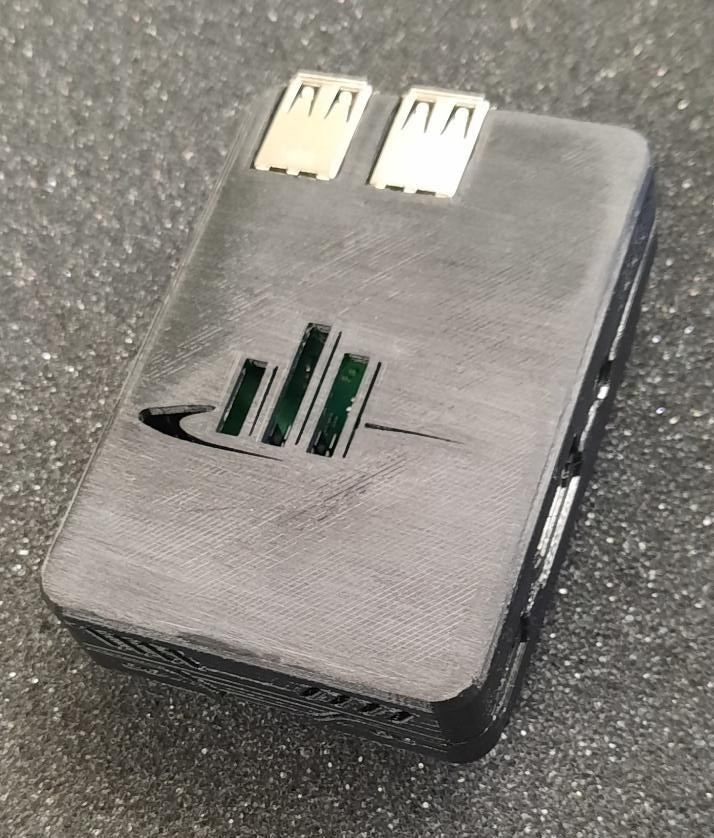
\includegraphics[width=4cm]{Pictures/PiGehaeuseVorne.jpeg}
\includegraphics[width=4cm]{Pictures/fig1.png}}
    \caption{The data connector mounted directly on the Kinova robot}
    \label{fig:dataConectorPic}
\end{figure}
The data connector can even be powered by the USB ports on the Kinova robot, so no additional power source is needed.\\
The Code is split into three main parts (Fig. \ref{fig:dataConectorStructure}).
\begin{figure}[htbp]
    \centerline{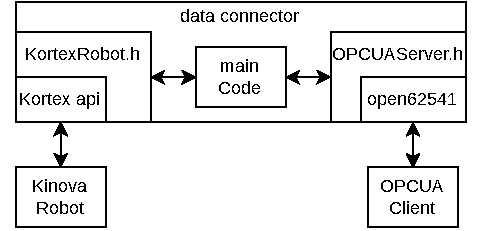
\includegraphics{Pictures/dataConectorStructure.pdf}}
    \caption{Code structure of the data connector}
    \label{fig:dataConectorStructure}
\end{figure}
One part is the communication to the robot via the Kortex api, the second part is the OPC-UA server with the open62541 library.
The main code part in the middle  starts a thread for the connection to the robot and a thread for the OPC-UA Server.
It also connects the data from from the robot class to the OPC-UA Server class.
So if the connector is used with another robot, it is enough to just write a new connection to the robot.
It is also possible to prepare the connection to a robot from a different manufacturer and let the main code detect what robot is connected.
This increases the flexibility of the data connector. 
% ToDo:
% syncronisation
% rapsi nicht auf der Oberflache bleiben
% batterie soc
% digialen zwilling vor dem kauf durch den Server simulation
\section{Performance Tests}
To ensure the data doesn't take to long from the robot to a client a series of performance tests are conducted.
These can be separate in two parts. 
First getting the data from the robot to the data connector and second get the data from the data connector to the client.
Every test is made with 5 samples. Every sample is the average speed of the first 1000 data requests.
\subsection{Getting data from the robot}
The Raspberry Pi 3B+ is directly connected to the Kinova robot via a ethernet cable.
With UDP as communication standard the Raspberry Pi can get the up to 1400 datasets per second from the Kinova robot (Fig. \ref{fig:KortexAPISpeed}).
That is even more than the 1000 datasets per second, that Kinova claims \cite{KortexUDP}.
\begin{figure}[htbp]
    \centerline{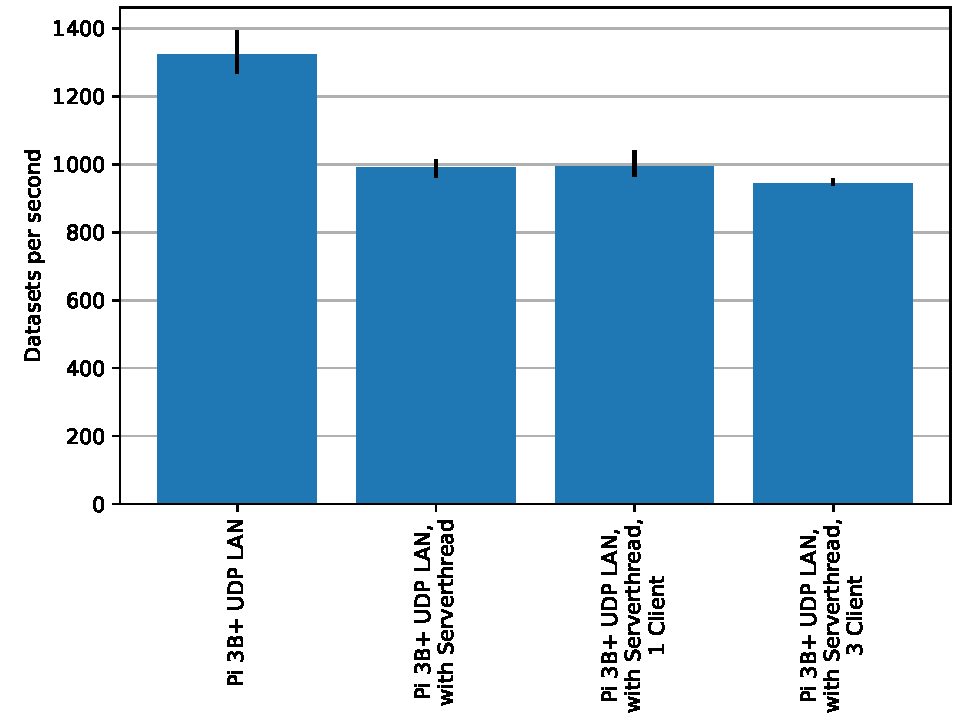
\includegraphics[width=8cm]{Pictures/KortexAPISpeed.pdf}}
    \caption{Frequency with which the Raspberry Pi 3B+ can get data from the Kinova arm}
    \label{fig:KortexAPISpeed}
\end{figure}
A dataset consists of all the data the robot has to offer. Thats over 50 data points.
Is the OPC-UA server is running parallel on the Raspberry Pi the frequency is lower, around 1kHz.
If one client is simultaneously requesting data from the OPC-UA server the frequency isn't really affected.
But if there are more clients then the frequency begins to drop slowly.
\subsection{Getting Data from the data connector}
To get the data from the data connector two different PCs are used. One midrange Laptop (Intel 11.Gen Core i7-1165G7, Realtek Semiconductor
RTL8152 Fast Ethernet Adapter) and an high end Tower PC (Intel 13.Gen Core i9-13900KF, Realtek Gaming R2.5GbE Family Controller).
The PCs and the data connector are all connected to a Router (tp-link Archer C80 AC1900 MU-MiMO).\\
\begin{figure}[htbp]
    \centerline{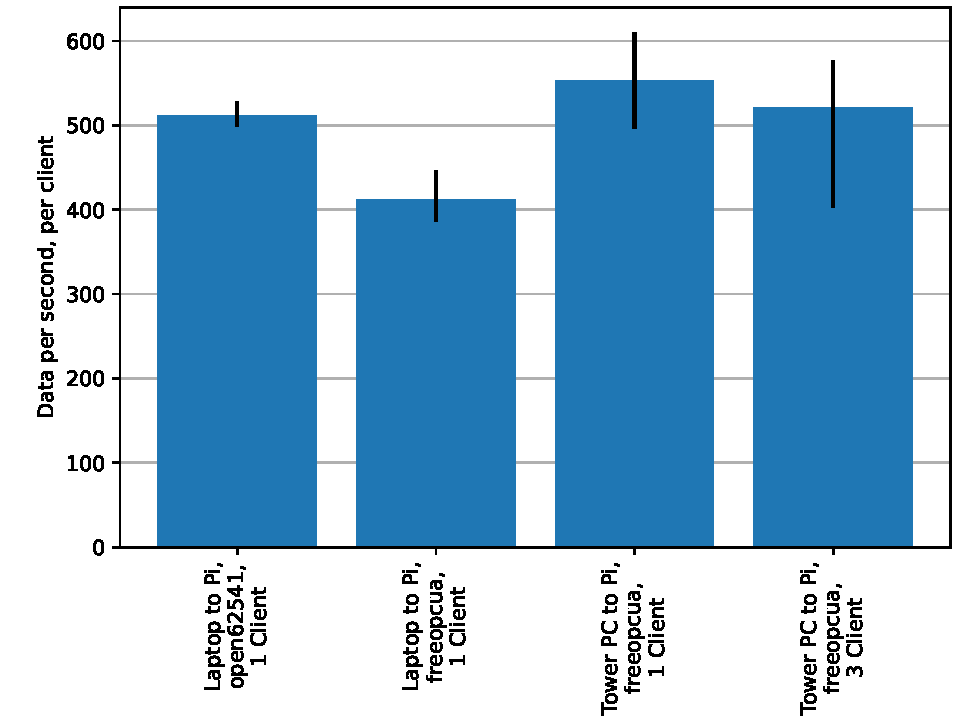
\includegraphics[width=8cm]{Pictures/OPCUASpeed1D.pdf}}
    \caption{Frequency with which data can be requested from the OPC-UA server}
    \label{fig:OPCUASpeed1D}
\end{figure}
In Fig. \ref{fig:OPCUASpeed1D} different libraries are used for the client to request one Value from the data connector.
On the Laptop the c-library open62541 is faster than the python library freeopcua.
On the Tower PC the python library is even faster than the c library on the Laptop.
If these results are compared to the ping between these PCs and the data connector (Fig. \ref{fig:PingDiagram}) it can be concluded that the python library on the Tower PC is running close to the actual limit of the network.\\
\begin{figure}[htbp]
    \centerline{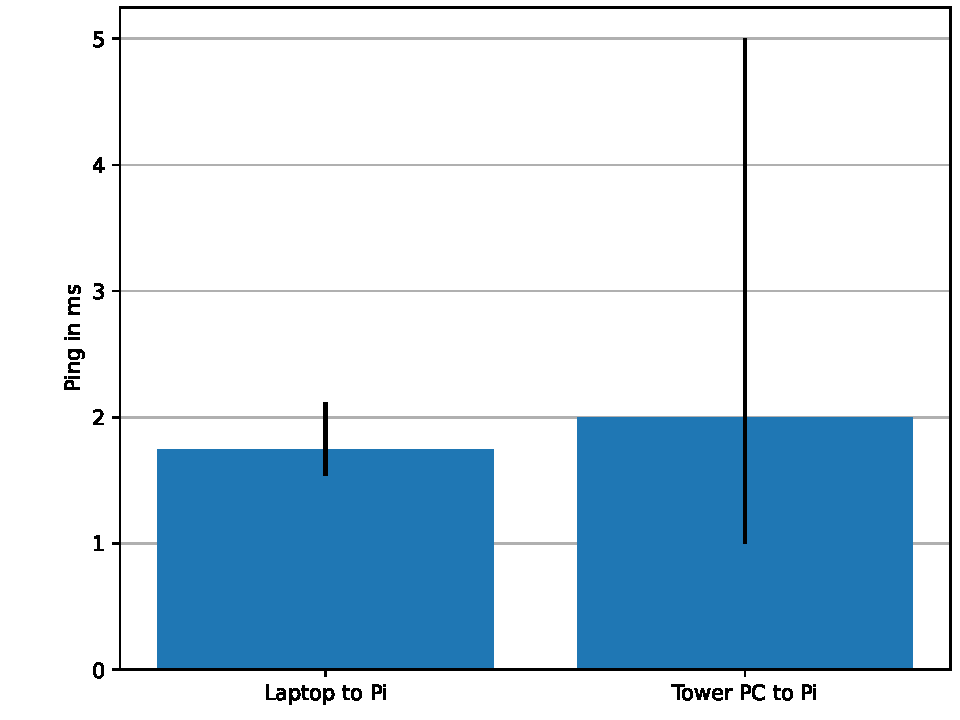
\includegraphics[width=8cm]{Pictures/PingDiagram.pdf}}
    \caption{Ping to the data connector}
    \label{fig:PingDiagram}
\end{figure}
If multiple clients are started in parallel on the Tower PC there is a slight decrease in the frequency with which the data can be requested from the data connector (Fig. \ref{fig:OPCUASpeed1D}).
\begin{figure}[htbp]
    \centerline{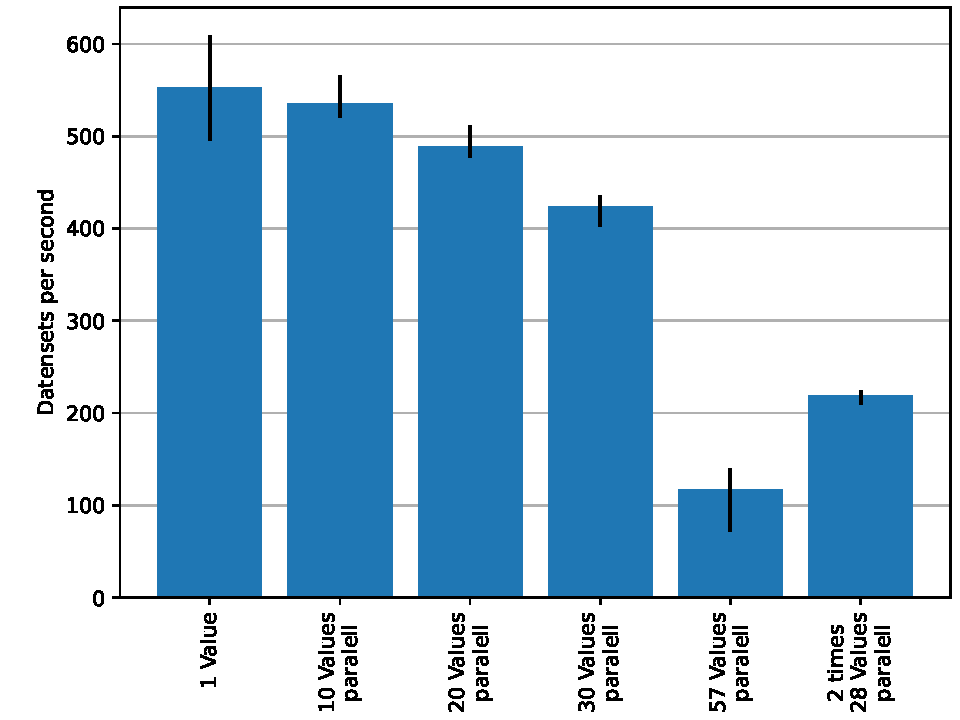
\includegraphics[width=8cm]{Pictures/OPCUAMultipleDatenAufEinmal.pdf}}
    \caption{Frequency with which different datasets can be requested from the OPC-UA server}
    \label{fig:OPCUAMultipleDatenAufEinmal}
\end{figure}
In the last test (Fig. \ref{fig:OPCUAMultipleDatenAufEinmal}) datasets with different amounts of values are requested from the data connector via the Tower PC using the python library.
The difference between 1 Value an 10 Values in one request is relative small (18 packages), between 10 and 20 Values this gap widens (47 packages) and between 20 and 30 it is even bigger (64 packages).
It is clearly not an linear decrease but also not an exponential one. 
Both the PC and the Raspberry Pi are using less than 20\% CPU so this isn't the bottleneck.
The size of the package gets bigger with every additional Value and there seems to be no limit at which the packages are split.
If all 57 Values are requested in one package its size is 2538 bytes.
This length is depending mostly of the name of the Values because the longer they are, the bigger the package.\\
The best way to request this many Values is in two packages with 28 and 29 Values each.
The frequency is half that of one 30 Value package but this is still nearly two times as fast as requesting all 57 Values in one package.
\section{Husky battery Soc}
\section{Digital twin}
The digital twin is build in Isaac Sim.
This is a simulation tool for robots which part of the NIVIDIA Omniverse.
In order to connecting to the OPC-UA server, a client is needed.
The best way to implement this is via an extension for Isaac Sim.
To reflect the modularity of robot system and the decentralized Network approach multiple different configurations of the robot system are created.
The extension has an Graphical User Interface (GUI) in which the configuration of the robot system can be chosen.
Independent form the chosen configuration it is also possible to choose to which OPC-UA server you want to connect.
This allows to test a robot configuration you don't have. 
For example it could be tested if the Husky will tip over when the Kinova arm does a specific movement, even if you don't have an Husky robot.
Just load an configuration with the Husky and an Kinova arm and connect to the Kinova arm.
The Kinova arm can now be moved with the controller and you can test any movement.\\
Furthermore it is possible to open a graph in which any data from the robot can be displayed.
So even the non-visible data can be visualized.
Even if you don't use one of the robots in the robot system it is still possible to connect to the robot to keep an eye on its vitals.\\
To make the digital twin more realistic you can choose in the GUI to load a 3D scan of the University as an environment for the digital twin (Fig. \ref{fig:CompareDigitalReal}).
\begin{figure}[htbp]
    \centerline{
\includegraphics[width=4cm]{Pictures/fig1.png}
\includegraphics[width=4cm]{Pictures/fig1.png}}
    \caption{Comparison of the digital twin (left) and the real robot (right)}
    \label{fig:CompareDigitalReal}
\end{figure}

\section{Remote access}
\newpage

\section*{Acknowledgment}

The preferred spelling of the word ``acknowledgment'' in America is without 
an ``e'' after the ``g''. Avoid the stilted expression ``one of us (R. B. 
G.) thanks $\ldots$''. Instead, try ``R. B. G. thanks$\ldots$''. Put sponsor 
acknowledgments in the unnumbered footnote on the first page.

\section*{References}

Please number citations consecutively within brackets \cite{b1}. The 
sentence punctuation follows the bracket \cite{b2}. Refer simply to the reference 
number, as in \cite{b3}---do not use ``Ref. \cite{b3}'' or ``reference \cite{b3}'' except at 
the beginning of a sentence: ``Reference \cite{b3} was the first $\ldots$''

Number footnotes separately in superscripts. Place the actual footnote at 
the bottom of the column in which it was cited. Do not put footnotes in the 
abstract or reference list. Use letters for table footnotes.

Unless there are six authors or more give all authors' names; do not use 
``et al.''. Papers that have not been published, even if they have been 
submitted for publication, should be cited as ``unpublished'' \cite{b4}. Papers 
that have been accepted for publication should be cited as ``in press'' \cite{b5}. 
Capitalize only the first word in a paper title, except for proper nouns and 
element symbols.

For papers published in translation journals, please give the English 
citation first, followed by the original foreign-language citation \cite{b6}.

\begin{thebibliography}{00}
\bibitem{OPCUA}https://opcfoundation.org/about/opc-technologies/opc-ua/
\bibitem{KortexUDP} Kinova, Kortex TransportClient classes, https://docs.kinovarobotics.com/kortex/linked\_md/cpp\_transport\_router\_session\_notif.html\#transportclient-classes, last checked 08.02.2024
\bibitem{b1} G. Eason, B. Noble, and I. N. Sneddon, ``On certain integrals of Lipschitz-Hankel type involving products of Bessel functions,'' Phil. Trans. Roy. Soc. London, vol. A247, pp. 529--551, April 1955.
\bibitem{b2} J. Clerk Maxwell, A Treatise on Electricity and Magnetism, 3rd ed., vol. 2. Oxford: Clarendon, 1892, pp.68--73.
\bibitem{b3} I. S. Jacobs and C. P. Bean, ``Fine particles, thin films and exchange anisotropy,'' in Magnetism, vol. III, G. T. Rado and H. Suhl, Eds. New York: Academic, 1963, pp. 271--350.
\bibitem{b4} K. Elissa, ``Title of paper if known,'' unpublished.
\bibitem{b5} R. Nicole, ``Title of paper with only first word capitalized,'' J. Name Stand. Abbrev., in press.
\bibitem{b6} Y. Yorozu, M. Hirano, K. Oka, and Y. Tagawa, ``Electron spectroscopy studies on magneto-optical media and plastic substrate interface,'' IEEE Transl. J. Magn. Japan, vol. 2, pp. 740--741, August 1987 [Digests 9th Annual Conf. Magnetics Japan, p. 301, 1982].
\bibitem{b7} M. Young, The Technical Writer's Handbook. Mill Valley, CA: University Science, 1989.
\end{thebibliography}
\vspace{12pt}
\color{red}
IEEE conference templates contain guidance text for composing and formatting conference papers. Please ensure that all template text is removed from your conference paper prior to submission to the conference. Failure to remove the template text from your paper may result in your paper not being published.

\end{document}

% \begin{table}[htbp]
% \caption{Table Type Styles}
% \begin{center}
% \begin{tabular}{|c|c|c|c|}
% \hline
% \textbf{Table}&\multicolumn{3}{|c|}{\textbf{Table Column Head}} \\
% \cline{2-4} 
% \textbf{Head} & \textbf{\textit{Table column subhead}}& \textbf{\textit{Subhead}}& \textbf{\textit{Subhead}} \\
% \hline
% copy& More table copy$^{\mathrm{a}}$& &  \\
% \hline
% \multicolumn{4}{l}{$^{\mathrm{a}}$Sample of a Table footnote.}
% \end{tabular}
% \label{tab1}
% \end{center}
% \end{table}
